\documentclass[onecolumn]{IEEEtran}
\usepackage[utf8]{inputenc}
\usepackage{graphicx}
\usepackage{amsmath}
\usepackage{array}
\usepackage{multirow}
\usepackage{hyperref}
\usepackage{xcolor}
\usepackage{float}
\usepackage{caption}
\usepackage{subcaption}

% Correct bad hyphenation here
\hyphenation{op-tical net-works semi-conduc-tor}

\begin{document}

% Paper title
\title{Optimasi Gerakan Robot Sepak Bola Menggunakan Kalman Filter pada Tracking Objek Berbasis YOLOv8}

\author{
    \IEEEauthorblockN{Fikri Rivandi\textsuperscript{1}, Feri Candra\textsuperscript{2}}
    \IEEEauthorblockA{\textsuperscript{1,2}Dept. of Informatics Engineering, Faculty of Engineering, Universitas Riau, Pekanbaru, Indonesia\\
    \textsuperscript{1}fikri.rivandi2583@student.unri.ac.id, \textsuperscript{2}feri@eng.unri.ac.id}
}

\maketitle

\begin{abstract}
Kontes Robot Sepak Bola Beroda Indonesia (KRSBI-Beroda) menuntut robot untuk melakukan deteksi dan \textit{tracking} bola secara \textit{real-time} di lingkungan yang dinamis. Metode \textit{tracking} berbasis deteksi tunggal seperti YOLOv8 seringkali terbentur pada keterbatasan perangkat keras (\textit{hardware}) dan gangguan visual seperti oklusi, yang menyebabkan gerakan robot menjadi tidak stabil. Penelitian ini mengusulkan optimasi sistem visi robot KRSBI-Beroda dengan mengintegrasikan algoritma \textit{You Only Look Once} versi 8 (YOLOv8) sebagai detektor objek dan \textit{Kalman Filter} sebagai estimator posisi prediktif. Pendekatan \textit{frame skipping} diimplementasikan untuk mengurangi beban komputasi pada perangkat laptop ASUS K401U, di mana YOLOv8 hanya dijalankan secara berkala, sementara \textit{Kalman Filter} memprediksi posisi bola di antara \textit{frame} deteksi. Hasil eksperimen menunjukkan peningkatan signifikan pada \textit{frame rate} (FPS) dari 13,6 menjadi 38,77. Sistem yang dioptimasi juga mampu menghilangkan \textit{tracking loss} (0 kejadian) pada skenario oklusi dan mengurangi waktu penyelesaian misi sebesar 62\% (dari 15,17 detik menjadi 5,76 detik). Integrasi ini terbukti mampu menstabilkan gerakan robot, mereduksi \textit{jitter}, dan meningkatkan keandalan sistem dalam pertandingan robot sepak bola.
\end{abstract}

\begin{IEEEkeywords}
KRSBI-Beroda, YOLOv8, Kalman Filter, \textit{Object Tracking}, \textit{Frame Skipping}, Robot Sepak Bola.
\end{IEEEkeywords}

\section{PENDAHULUAN}

Perkembangan teknologi \textit{computer vision} dan \textit{deep learning} telah mendorong kemajuan pesat dalam bidang robotika otonom, khususnya pada ajang Kontes Robot Indonesia (KRI) kategori Kontes Robot Sepak Bola Beroda Indonesia (KRSBI-Beroda) \cite{Kusumoputro2024}. Dalam kompetisi ini, robot dituntut untuk mampu mendeteksi dan melacak (\textit{tracking}) pergerakan bola secara \textit{real-time} untuk melakukan manuver \textit{dribbling} dan mencetak gol. Kegagalan dalam \textit{tracking} bola, baik karena keterbatasan komputasi maupun gangguan oklusi, dapat berakibat fatal pada performa robot.

Tim \textit{Engineering Robotic Club} (ERC) Universitas Riau sebelumnya mengandalkan metode \textit{HSV color filtering} untuk deteksi bola. Metode ini ringan namun sangat sensitif terhadap perubahan intensitas cahaya, sehingga tidak andal dalam kondisi lapangan yang dinamis \cite{Nanda2023}. Seiring perkembangan, metode berbasis \textit{Convolutional Neural Network} (CNN) seperti \textit{You Only Look Once} (YOLO) diadopsi untuk meningkatkan akurasi deteksi \cite{Farhan2025}. YOLO mampu mendeteksi objek dengan presisi tinggi meskipun dalam variasi pencahayaan, namun implementasinya pada perangkat keras terbatas seperti laptop ASUS K401U milik robot ERC UNRI menimbulkan masalah baru: beban komputasi yang tinggi menyebabkan \textit{frame rate} (FPS) rendah dan \textit{lag} \cite{Miharja2025}. Akibatnya, robot sering kehilangan jejak bola saat bergerak cepat atau saat bola tertutup sebagian (oklusi).

Untuk mengatasi \textit{trade-off} antara akurasi deteksi dan efisiensi komputasi, penelitian ini mengusulkan integrasi YOLOv8 dengan \textit{Kalman Filter}. \textit{Kalman Filter} adalah algoritma estimator rekursif yang ringan dan mampu memprediksi keadaan sistem dinamis berdasarkan data sebelumnya \cite{Sholehurrohman2023}. Dengan menerapkan strategi \textit{frame skipping}, detektor YOLO tidak perlu dijalankan di setiap \textit{frame}; sebaliknya, \textit{Kalman Filter} mengambil alih tugas estimasi posisi di antara \textit{frame} deteksi. Pendekatan ini terbukti meningkatkan efisiensi komputasi dan ketahanan terhadap oklusi \cite{Taylor2016, Takura2021}. Tujuan dari penelitian ini adalah mengembangkan sistem \textit{tracking} yang lebih stabil dan responsif pada robot KRSBI-Beroda dengan memanfaatkan sinergi antara YOLOv8 dan \textit{Kalman Filter}.

\section{METODOLOGI PENELITIAN}

Penelitian ini menggunakan pendekatan eksperimental kuantitatif dengan membandingkan dua sistem: \textbf{Sistem \textit{Baseline}} (YOLOv8 murni tanpa \textit{frame skipping}) dan \textbf{Sistem \textit{Optimized}} (YOLOv8 + \textit{Kalman Filter} dengan \textit{frame skipping}). Diagram alur metodologi penelitian dapat dilihat pada Gambar \ref{fig:flowchart}.

\begin{figure}[H]
\centering
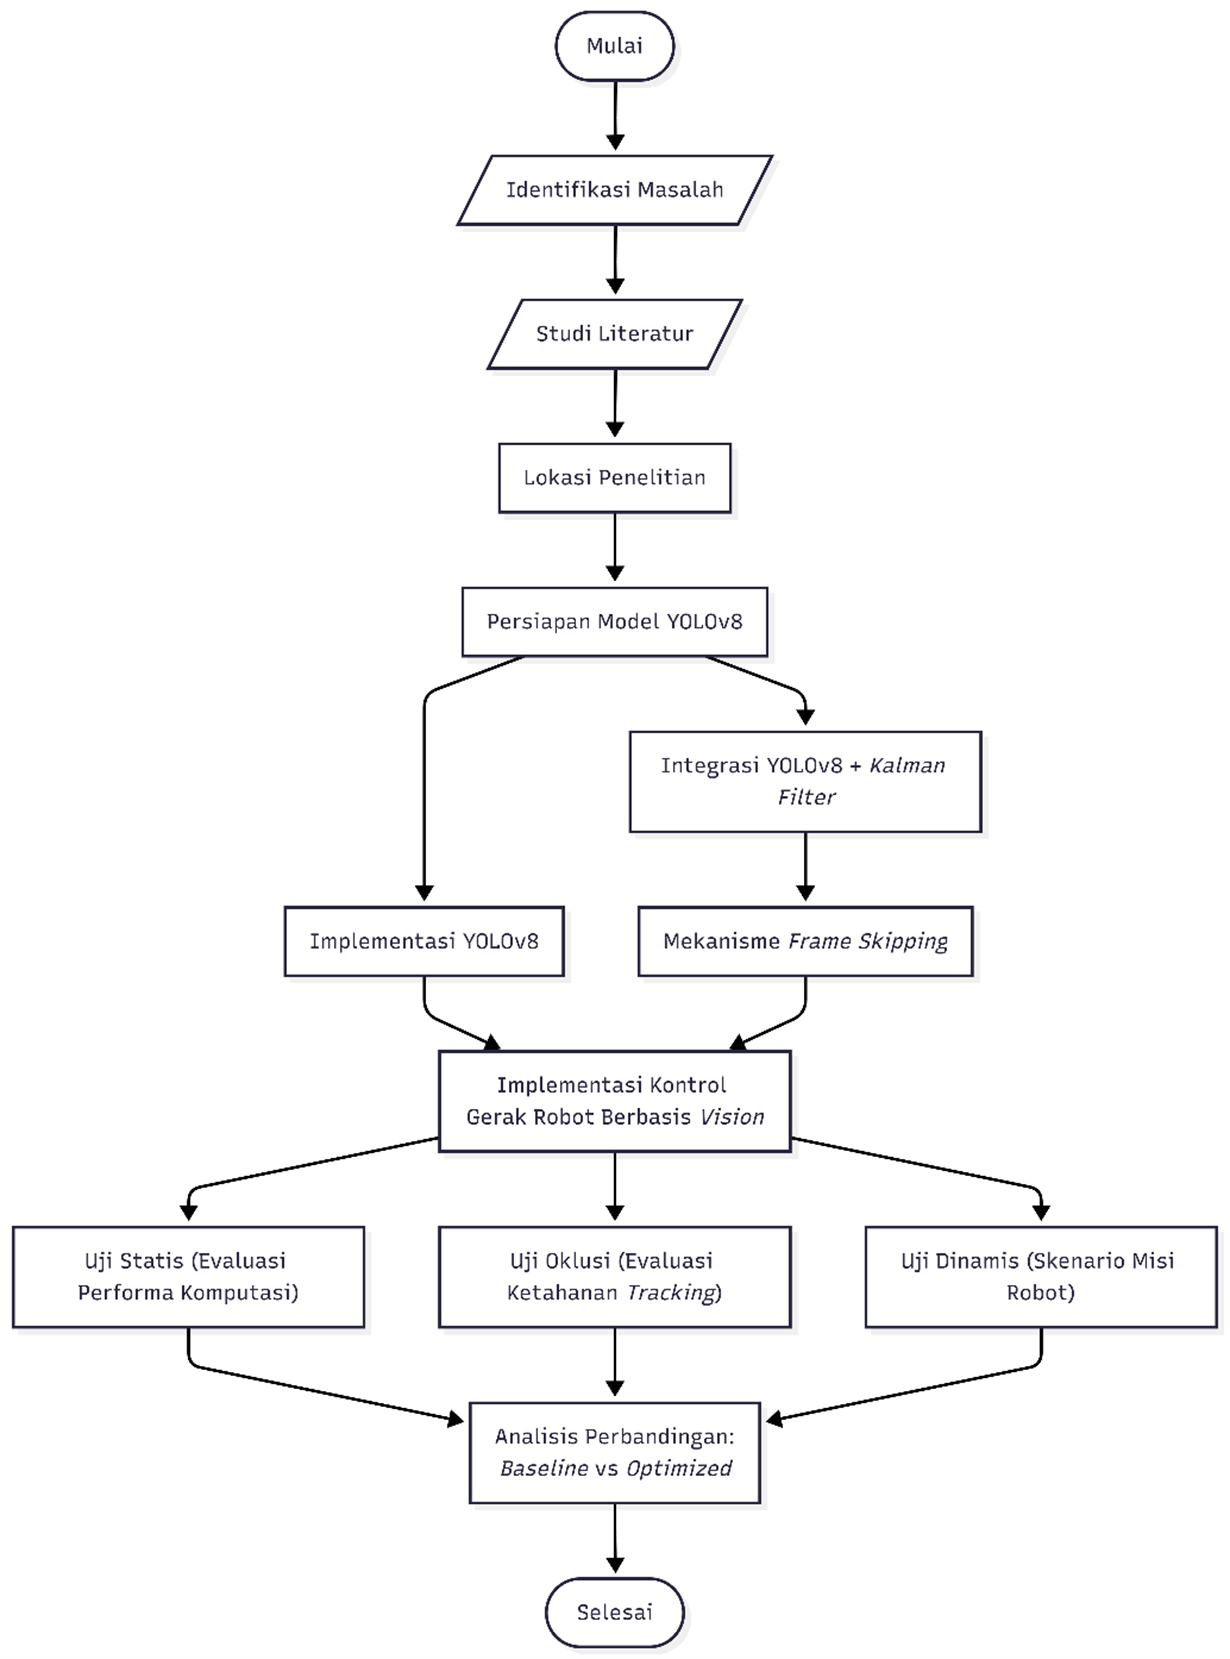
\includegraphics[width=\linewidth]{metodologipenelitian.png}
\caption{Diagram Alur Metodologi Penelitian}
\label{fig:flowchart}
\end{figure}

\subsection{Implementasi Sistem Optimasi \textit{Kalman Filter}}
Pada sistem \textit{optimized}, arsitektur \textit{tracking} dirancang untuk mengurangi beban komputasi tanpa mengorbankan kontinuitas \textit{tracking}. Sistem tidak menjalankan deteksi YOLOv8 pada setiap \textit{frame}, melainkan menerapkan \textit{frame skipping} dengan interval 3 \textit{frame} ($SL = 3$). Artinya, inferensi YOLOv8 dilakukan pada \textit{frame} ke-1, sedangkan pada \textit{frame} ke-2 dan ke-3 sistem mengandalkan prediksi dari \textit{Kalman Filter}.

Vektor keadaan (\textit{state vector}) $X$ didefinisikan sebagai:
\[
X = [x, y, v_x, v_y, w, h]^T
\]
di mana $(x, y)$ adalah koordinat pusat bola, $(v_x, v_y)$ adalah kecepatan objek, serta $(w, h)$ adalah dimensi \textit{bounding box}. Model gerak yang digunakan adalah \textit{Constant Velocity} dengan matriks transisi $F$ dan matriks observasi $H$ yang hanya membaca $(x, y, w, h)$ karena YOLO tidak menyediakan data kecepatan secara langsung.

Ketika YOLO dijalankan, data koordinat bola $(x, y)$ digunakan sebagai vektor pengukuran $Z$ untuk melakukan koreksi (\textit{update step}) pada \textit{Kalman Filter}. Sebaliknya, pada \textit{frame} yang dilompati, \textit{Kalman Filter} melakukan prediksi (\textit{predict step}) untuk menghasilkan estimasi posisi bola.

\subsection{Evaluasi Sistem}
Pengujian dilakukan dalam tiga skenario utama untuk mengukur efektivitas optimasi:
\begin{enumerate}
    \item \textbf{Uji Statis:} Mengukur rata-rata \textit{Frames Per Second} (FPS) selama 30 detik (10 kali repetisi).
    \item \textbf{Uji Oklusi:} Menguji ketahanan \textit{tracking} terhadap gangguan visual (Ringan 30\%, Sedang 60\%, Sesaat 1-2 detik) dengan parameter \textit{Tracking Loss Count} dan Durasi Kehilangan.
    \item \textbf{Uji Dinamis:} Mensimulasikan misi mencetak gol untuk mengukur waktu penyelesaian misi dan stabilitas gerakan (\textit{jitter}).
\end{enumerate}

\section{HASIL DAN PEMBAHASAN}

\subsection{Analisis Performa Komputasi}
Berdasarkan hasil uji statis yang dirangkum pada Tabel \ref{tab:fps}, sistem \textit{optimized} berhasil meningkatkan rata-rata FPS secara drastis.

\begin{table}[H]
\centering
\caption{Perbandingan Rata-rata FPS}
\label{tab:fps}
\begin{tabular}{|c|c|c|}
\hline
\textbf{Repetisi} & \textbf{Sistem Baseline (FPS)} & \textbf{Sistem Optimized (FPS)} \\
\hline
1 & 13.91 & 41.28 \\
2 & 14.34 & 36.29 \\
3 & 13.54 & 37.61 \\
4 & 13.73 & 43.16 \\
5 & 13.52 & 34.38 \\
6 & 13.48 & 35.30 \\
7 & 12.68 & 40.05 \\
8 & 12.52 & 38.83 \\
9 & 15.09 & 44.00 \\
10 & 13.21 & 36.81 \\
\hline
\textbf{Rata-rata} & \textbf{13,60} & \textbf{38,77} \\
\hline
\end{tabular}
\end{table}

Peningkatan FPS hingga 185\% ini terjadi karena \textit{Kalman Filter} secara signifikan lebih ringan secara komputasi ($O(n^2)$ matriks sederhana) dibandingkan inferensi jaringan saraf YOLOv8 yang memakan sumber daya CPU/GPU secara intensif. Dengan FPS di atas 30, sistem memenuhi syarat \textit{real-time} dan robot dapat bereaksi lebih cepat terhadap pergerakan bola.

\subsection{Ketahanan Terhadap Oklusi}
Pada Tabel \ref{tab:oklusi}, sistem \textit{baseline} kehilangan jejak bola secara total saat oklusi sedang dan sesaat. Sebaliknya, sistem \textit{optimized} mencatatkan \textbf{0 (nol)} \textit{tracking loss}. 

\begin{table}[H]
\centering
\caption{Perbandingan \textit{Tracking Loss} pada Uji Oklusi}
\label{tab:oklusi}
\begin{tabular}{|c|c|c|c|c|}
\hline
\multirow{2}{*}{\textbf{Skenario}} & \multicolumn{2}{c|}{\textbf{Baseline}} & \multicolumn{2}{c|}{\textbf{Optimized}} \\
\cline{2-5}
 & \textit{Loss Count} & Durasi (s) & \textit{Loss Count} & Durasi (s) \\
\hline
Oklusi Ringan & 0 & 0 & 0 & 0 \\
Oklusi Sedang & 96 & 13,94 & 0 & 0 \\
Oklusi Sesaat & 6 & 2,89 & 0 & 0 \\
\hline
\end{tabular}
\end{table}

Hal ini membuktikan bahwa \textit{Kalman Filter} berfungsi sebagai "memori spasial" bagi robot. Saat bola tertutup dan YOLO gagal mendeteksi, \textit{Kalman Filter} tetap memproyeksikan lintasan bola berdasarkan estimasi kecepatan $(v_x, v_y)$ sebelumnya. Kemampuan ini sangat krusial untuk menghindari kebingungan navigasi saat robot bertabrakan dengan lawan.

\subsection{Stabilitas Gerakan dan Waktu Misi}
Data log perintah gerak robot menunjukkan penurunan \textit{jitter} yang signifikan. Total perintah koreksi arah (\textit{putarKiri/Pelan} dan \textit{putarKanan/Pelan}) pada sistem \textit{optimized} turun drastis dari 74 kali menjadi hanya 23 kali selama 5 kali pengujian. Reduksi \textit{jitter} ini berdampak langsung pada efisiensi waktu penyelesaian misi.

\begin{table}[H]
\centering
\caption{Rata-rata Waktu Penyelesaian Misi}
\label{tab:waktu}
\begin{tabular}{|c|c|c|}
\hline
\textbf{Repetisi} & \textbf{Baseline (detik)} & \textbf{Optimized (detik)} \\
\hline
1 & 12,400 & 7,254 \\
2 & 19,277 & 5,350 \\
3 & 12,986 & 5,987 \\
4 & 19,139 & 5,615 \\
5 & 12,057 & 4,638 \\
\hline
\textbf{Rata-rata} & \textbf{15,171} & \textbf{5,768} \\
\hline
\end{tabular}
\end{table}

Robot \textit{optimized} mampu menyelesaikan misi mencetak gol 62\% lebih cepat. Gerakan robot menjadi lebih halus dan linear karena estimasi \textit{Kalman Filter} menghilangkan fluktuasi koordinat yang biasanya muncul akibat \textit{noise} deteksi YOLO atau perubahan pencahayaan sesaat.

\section{KESIMPULAN}

Berdasarkan hasil penelitian, integrasi \textit{Kalman Filter} pada sistem \textit{tracking} YOLOv8 terbukti efektif mengoptimasi gerakan robot KRSBI-Beroda. Kesimpulan yang diperoleh adalah:
\begin{enumerate}
    \item Sistem \textit{optimized} berhasil meningkatkan rata-rata FPS dari 13,6 menjadi 38,77, mengatasi bottleneck komputasi pada laptop ASUS K401U.
    \item \textit{Kalman Filter} memberikan ketahanan sempurna terhadap oklusi (0\% \textit{tracking loss}), memastikan robot tidak kehilangan arah saat bola terhalang.
    \item Stabilitas gerakan meningkat secara signifikan dengan reduksi \textit{jitter} perintah gerak, yang menghasilkan penyelesaian misi 62\% lebih cepat.
\end{enumerate}
Untuk pengembangan selanjutnya, disarankan menggunakan perangkat \textit{edge computing} seperti NVIDIA Jetson untuk menjalankan YOLO di setiap \textit{frame} serta mengeksplorasi \textit{Extended Kalman Filter} (EKF) untuk memodelkan dinamika bola yang non-linier.

\begin{thebibliography}{00}

\bibitem{Kusumoputro2024} B. Kusumoputro \textit{et al.}, ``Pedoman Kontes Robot Indonesia (KRI) Pendidikan Tinggi Tahun 2024,'' Balai Pengembangan Talenta Indonesia, Pusat Prestasi Nasional, Kemdikbudristek, 2023.

\bibitem{Nanda2023} B. M. Nanda, S. Siregar, and M. I. Sani, ``Implementasi Object Detection Pada Robot Sepak Bola Beroda Berbasis Kamera Omnidirectional Menggunakan OpenCV,'' \textit{J. Tek.}, vol. 9, no. 4, pp. 2064–2068, 2023.

\bibitem{Farhan2025} T. M. Farhan and F. Candra, ``CNN-Based Ball and Goal Detection for KRSBI Robot with Omnidirectional Camera,'' \textit{J. Informatics, Electrical, Electronics, and Physical Engineering}, vol. 08, no. 02, pp. 86-98, 2025.

\bibitem{Miharja2025} M. Surya, A. N. Toscany, C. Saputra, Y. Pratama, and M. I. Bustami, ``Penggunaan YOLO Untuk Deteksi Robot Dan Gawang Pada Robot Sepak Bola Beroda,'' \textit{Indones. J. Comput. Sci.}, vol. 14, no. 1, pp. 1055–1070, 2025.

\bibitem{Sholehurrohman2023} R. Sholehurrohman, M. R. Habibi, I. S. Ilman, R. Taufiq, and M. Muhaqiqin, ``Analisis Metode Kalman Filter, Particle Filter dan Correlation Filter Untuk Pelacakan Objek,'' \textit{Komputika J. Sist. Komput.}, vol. 12, no. 2, pp. 21–28, 2023.

\bibitem{Taylor2016} L. E. Taylor, M. Mirdanies, and R. P. Saputra, ``Optimized Object Tracking Technique Using Kalman,'' \textit{J. Mechatronics, Electr. Power, Veh. Technol.}, vol. 07, pp. 57–66, 2016.

\bibitem{Takura2021} K. Takura, Y. Arita, and S. H. Oaki, ``Automatic pear and apple detection by videos using deep learning and a Kalman filter,'' \textit{OSA Continuum}, vol. 4, no. 5, pp. 1688–1695, 2021.

\end{thebibliography}

% Biographies (Opsional)
% ----------------- BIOGRAPHY DENGAN FOTO -----------------
\section*{BIOGRAFI PENULIS}

\vspace{0.5cm}

\noindent
\begin{minipage}{0.25\textwidth}
    \centering
    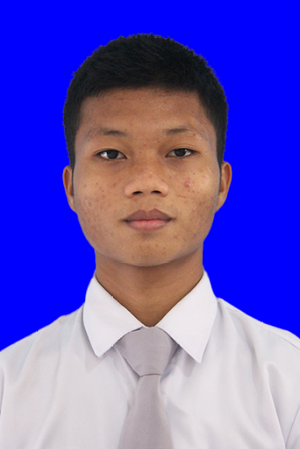
\includegraphics[width=3cm,height=3cm,keepaspectratio]{foto_fikri.png} \\
    \small \textbf{Fikri Rivandi}
\end{minipage}
\hfill
\begin{minipage}{0.7\textwidth}
    \small
    Lahir di Rokan Hilir, Riau. Mahasiswa Program Studi Teknik Informatika, Fakultas Teknik, Universitas Riau angkatan 2022. Selama perkuliahan aktif di \textit{Engineering Robotic Club} (ERC) UNRI dan berfokus pada bidang Robotika, \textit{Computer Vision}, Kecerdasan Buatan, serta \textit{Embedded System}. Penelitian yang dilakukan berfokus pada optimasi sistem visi robot sepak bola beroda menggunakan pendekatan \textit{deep learning} dan \textit{Kalman Filter}.
\end{minipage}

\vspace{1cm}

\noindent
\begin{minipage}{0.25\textwidth}
    \centering
    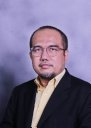
\includegraphics[width=3cm,height=3cm,keepaspectratio]{foto_feri_candra.jpg} \\
    \small \textbf{Feri Candra, S.T., M.T., Ph.D.}
\end{minipage}
\hfill
\begin{minipage}{0.7\textwidth}
    \small
    Dosen di Program Studi Teknik Informatika, Fakultas Teknik, Universitas Riau. Menyelesaikan pendidikan S1 di Institut Sains dan Teknologi Nasional, S2 di Universitas Indonesia, dan S3 di Universiti Teknologi Malaysia. Memiliki keahlian dan minat penelitian di bidang \textit{Machine Learning}, \textit{Computer Vision}, Robotika, dan \textit{Internet of Things} (IoT). Aktif sebagai pembimbing tim robotika ERC UNRI dan reviewer di berbagai jurnal nasional maupun internasional.
\end{minipage}

\end{document}